\section{Metode}
\subsection*{Utstyr}
\begin{itemize}
    \item Telefoner med Phyphox
    \item Telefonholder
    \item Trefot
    \item Vater
\end{itemize}
Det ble foretatt målinger med Djupviks iPhone SE, Jakobsens Samsung Galaxy A40 og Aakres iPhone 13. 

\subsection{Referansepunkter og målelokasjon}
Det ble gjort målinger med 2 ulike referansepunkt for å få et større datagrunnlag. De valgte referansepunktene var spiret til Nidarosdomen og Tyholttårnet fordi disse var lette å sikte seg inn på i tillegg til å være et godt stykke unna målelokasjonen (se figur \ref{fig:angle_north}). 
Målingene ble utført på vestre siden av broen som krysser Eidsvolls gate langs Øvre alle. 

Koordinatene til referansepunktene ble bestemt med å klikke på punktene på Google Maps (satelitt-bilder). 
Koordinatene til målelokasjonen ble målt ved hjelp av phyphox' verktøy for lokasjonsmåling \cite{phyphox}. Telefonens GPS-sensor ble kalibrert ved at telefonen ble flyttet rundt målelokasjonen. 
Deretter ble telefonen plassert i ro i telefonholderen. 
Lokasjonsdata ble eksportert i \kode{.csv}-format.

\begin{figure}[h!]
    \centering
    
\includegraphics[width=0.66\textwidth, trim={0 100 0 0}, clip]{img/angle_north.pdf}
    \caption{
    Skisse av målelokasjon ($A$) og to referansepunkter ($B$ og $C$) samt vinkelene mellom disse og geografisk nord.}
    \label{fig:angle_north}
\end{figure}

\subsection{Måling av magnetfelt og oppsett}
En trefot med en plattform for telefonene ble brukt, hvor telefonene ble plassert i en telefonholder. For å gi riktig retning på telefonene, ble det plassert ett vater langsmed telefonholderen (se figur \ref{fig:med_vater}). Vateret ble så brukt som siktemiddel slik at telefonholderen, og dermed $-x$-aksen til telefonens referansesystem \ref{fig:telf_akser}, lå i retning av referansepunktet. Vi får da at $\psi = -180$\textdegree\ i ligning \eqref{eq:Deklinasjon}. Deretter ble plattformens inklinasjon justert slik at telefonen la horisontalt ved hjelp av vateret.

Før hver måling ble telefonene kalibrert ved å rotere den rundt alle tre aksene. Deretter ble telefonene plassert i telefonholderen og ble liggende omkring $30$ sekunder. Dataene ble så eksportert til \kode{.csv}-format. 

Måling med Nidarosdomen som referansepunkt ble gjennomført først. Det ble gjennomført et målesett (en måling med hver telefon). Deretter ble plattformen stilt inn på nytt med Tyholttårnet som referansepunkt. Det ble gjort målinger med flymodus aktivert og etter å ha gjort en omstart av telefonene for å sjekke om dette kunne ha innvirkning på resultatene. Målingene med flymodus ble gjennomført ved at telefonene ble satt i flymodus, kalibrert og dermed satt i telefonholderen. Målingene etter omstart ble gjennomført ved at telefonene ble startet på nytt, kalibrert og så plassert i telefonholderen.



\begin{figure}[h!]
    \centering
\begin{subfigure}{.47\textwidth}
    \includegraphics[width=\textwidth]{img/Plattform med vater.pdf}
    \caption{Figuren viser oppsettet for måling før telefonen ble plassert i telefonholderen. Vateret er siktemiddel for oppsettet.}
    \label{fig:med_vater}
\end{subfigure}\hfill\begin{subfigure}{.47\textwidth}
    \includegraphics[width=\textwidth]{img/Plattform med telefoni.pdf}
    \caption{Skisse av telefon under måling. Skissen viser også koordinatsystemet, angitt med $\hat{x}, \hat{y}, \hat{z}$, som benyttes til analysen.}
    \label{fig:telf_akser}
\end{subfigure}
\end{figure}





\subsubsection{Analyse av data}
Rådata for magnetfeltet og koordinatene til målelokasjonen ble gruppert for målesett og telefon.
Inklinasjonen ble bestemt ved bruke \eqref{eq:inclination} på hvert datasett, samt bruke funksjonene 
\href{https://numpy.org/doc/stable/reference/generated/numpy.mean.html#numpy.mean}{\kode{numpy.mean}}, 
\href{https://numpy.org/doc/stable/reference/generated/numpy.median.html#numpy-median}{\kode{numpy.median}} og 
\href{https://docs.scipy.org/doc/scipy/reference/generated/scipy.stats.tstd.html#scipy.stats.tstd}
{\kode{sympy.stats.tstd}} for å finne gjennomsnittet, medianen og 
standardavviket.
Deretter ble vinkelen mellom referansepunkt og geografisk nord ($\theta$) regnet ut for hver telefon ved å 
bruke \kode{geodesic.Geodesic.WGS84.Inverse()} fra geographiclib-biblioteket.
Innsatt i \eqref{eq:Deklinasjon} gir dette deklinasjonen for hvert målesett.
Deretter ble alle dataene samlet i et målesett, og analysert i sin helhet med analysemetoden som ble brukt 
for hvert enkelt datasett beskrevet over.
På grunn av stort avvik fra de andre målesettene ble måledataene til iPhone 13 for Nidarosdomen filtrert ut. En ny analyse ble så gjennomført. 